\documentclass[12pt]{article}

% My standard included packages
\usepackage{fontspec}
\usepackage{setspace}           % Allows easy changes to line spacing 
\usepackage{graphicx}           % Allows including of graphics files
\usepackage{amsmath}            % Additional math capabilities
\usepackage{marginnote}         % Used with todonotes package
\usepackage{datetime}           % Allows formatting of date and
\usepackage{dsfont}
\usdate                         % Use usual LaTeX date layout
\usepackage{enumitem}           % List formatting commandsen list items 
%\usepackage{bbm}                % Indicator function
\usepackage{subfigure}          % Create numbered and captioned subfigures
\usepackage{rotating}           % Create landscape tables and figures
\usepackage[dvipsnames]{xcolor} % Refer to colors by name
\usepackage[colorlinks=true,urlcolor=blue,linkcolor=Black,citecolor=RedViolet]{hyperref}           % URLS and hyperlinks
\usepackage{float}              % Activate [H] option to place figure HERE
\graphicspath{{graphics/}}
\makeatletter
\def\@xfootnote[#1]{%
  \protected@xdef\@thefnmark{#1}%
  \@footnotemark\@footnotetext}
\makeatother
\usepackage[style=apa,backend=biber,sorting=nyt]{biblatex}
\addbibresource{ref.bib}
\linespread{1.3}
\setromanfont{Helvetica}
\author{}
\date{}
\title{Estimation of algorithmic liquidity trading intensity}
\begin{document}
\setlist{noitemsep}             % Remove space betwe time
\maketitle
\newpage
\tableofcontents
\newpage

\section{Introduction}\label{sec:intro}
With algorithmic trading (AT) comprising over 50\% of dollar trading volume in developed countries, it becomes more and more important to accurately estimate and study its effect on markets. But, due to a number of reasons, this task may prove difficult without proper data, hindering overall progress in AT-related research. 
%\footnote{The estimate made in accordance with Hendershott and Riordan (2011)} deleted from above due to page size issues
Several papers overcome this problem using various indirect measures of AT. For example, in Hendershott, Jones and Menkveld (2011) the instrumental variable approach is used in order to estimate AT effect on volatility and liquidity and establish a causal link between AT and market changes. They use trading volume per electronic message (both per unit of time) multiplied by $-1$ as an instrumental variable for AT. The intuition behind this measure is that algorithms slice large orders and trade them chunk by chunk throughout a period of time thus reducing the above-mentioned ratio. Thus, as AT activity increases, average transaction size decreases. This measure is then multiplied by $-1$ to get positive correlation between AT activity and the instrument.

In this study, we consider large liquidity traders who need to buy or sell large amounts of assets in a limited period of time. These traders are likely to slice their full orders into chunks and trade them throughout this time frame. This study aims to illustrate an approach that uses intuition similar to one in HJM (2011). We introduce a measure of liquidity trading as a probability of a particular agent being either a liquidity or a noise trader. The key feature of this approach is the usage of autocorrelation function of trading volume as a mean to measure the above-mentioned probability. We show that, given that we know the exact distributions of traders' strategies and underlying random variables, one can infer the probability of an agent being a liquidity trader from the functional form of sampled ACF.
\newpage

\section{Market Model}\label{sec:model}
We consider the following problem. Suppose that a trader must move his or her portfolio from state A to state B during the time period of $T$. Assuming that his or her target (the difference between states) is large enough, this trader can be roughly identified as institutional. Due to certain reasons, such traders cannot (or don't want to) execute their orders right away. The main reason is that the implementation shortfall (i.e., the costs of implementing a certain trading strategy) will be tremendous if one chooses to execute a large order at once because of a huge price impact of transactions this large. Thus, such orders are likely to be sliced and traded chunk by chunk throughout the entire time period T.

Obviously, knowing the functional form of a trade trajectory, time $T$, and target size $X$, one can trace the trade history of a certain agent via trade log. But, even without specific knowledge about the above-mentioned parameters, it is possible to estimate the presence of such trading because transactions will be (under certain assumptions) autocorrelated. Thus, it might be possible to measure liquidity trading intensity relying on ACF of trading volume.

Consider the following market model: during every \textit{i\textsuperscript{th}} time period of length $\tau$ a Poisson random number (with expected value $l$) of traders arrive on the market and start trading. There are 2 types of traders: institutional or liquidity traders (LT) (appear with probability $\theta> 0$), and noise traders (NT) (appear with probability $1-\theta$). The difference between these 2 types of traders is as follows: noise traders' target sizes are normally distributed with mean 0 and variance $\sigma^2_{NT}$ and constant execution time T=1, while liquidity traders' target sizes $Q_i$ are normally distributed with mean 0 and variance $\sigma^2_{LT}$ and their execution time T is randomly distributed. 

There are certain assumptions about the trader's interaction within the market: 
\begin{enumerate}
\item traders' strategies are independent given public signal $\xi$. This assumption is made because certain signals such as price changes or news announcements are likely to trigger trading. If this happens, one can see correlations in data that are not due to true dependence of traders' strategies, but because of omission of such signals;
\item $E(y_{it}\vert\xi_0)=0$, that is, the expected trade size of the \textit{i\textsuperscript{th}} trader at time \textit{t} is equal to zero given $\xi_0$;
\item traders' strategies are homogenous.
\end{enumerate}
The following calculations are based on these 3 assumptions. 

Thus, autocovariance $Cov(Y_t,Y_{t+\Delta}\vert\xi_0)$ of trading volume in this market is:
\begin{equation}\label{one}
\begin{gathered}
E(Y_t\cdot Y_{t+\Delta}\vert\xi_0)=E((\sum\limits_{i=1}^{H_t}y_{it}+\sum\limits_{i=1}^{N_t}z_{it})\cdot
(\sum\limits_{j=1}^{H_{t+\Delta}}y_{it+\Delta}+\sum\limits_{j=1}^{N_{t+\Delta}}z_{it+\Delta})\vert\xi_0)\\
=E(\sum\limits_{i=1}^{H_t}y_{it}\cdot\sum\limits_{j=1}^{H_{t+\Delta}}y_{it+\Delta}\vert\xi_0)
\end{gathered}
\end{equation}
% probably write about z_it as well?
% change indices?
where $Y_t$ is trading volume at time $t$, $y_{it}$ is the size of the $i_{th}$ trader's transaction at time $t$, $H_t$ and $N_t$ is the number of liquidity and noise traders present on the market by the time $t$ respectively (note that $H_t$ and $N_t$ are just different "flows" of a single Poisson process), and $\Delta$ is the chosen lag. Because we assume that traders are independent from each other, we can decompose the formula above into 2 expected values\footnote[$\ast$]{Here and below $E(•)$ implies $E(•\vert\xi_0)$ unless explicitly stated otherwise.}:
\begin{equation}\label{two}
\begin{gathered}
E(\sum\limits_{i=1}^{H_t}y_{it}\cdot\sum\limits_{j=1}^{H_{t+\Delta}}y_{it+\Delta})=
E(\sum\limits_{i=1}^{H_t}y_{it}\cdot\sum\limits_{j=1}^{H_{t}}y_{it+\Delta})+
E(\sum\limits_{i=1}^{H_t}y_{it}\cdot\sum\limits_{j=H_t+1}^{H_{t+\Delta}}y_{it+\Delta})\\=
E(\sum\limits_{i=1}^{H_t}y_{it}\cdot\sum\limits_{j=1}^{H_{t}}y_{it+\Delta})+
E(\sum\limits_{i=1}^{H_t}y_{it})\cdot E(\sum\limits_{j=H_t+1}^{H_{t+\Delta}}y_{it+\Delta})
\\=E(\sum\limits_{i=1}^{H_t}y_{it}\cdot\sum\limits_{j=1}^{H_{t}}y_{it+\Delta})=
E(\sum\limits_{i=1}^{H_t}y_{it}\cdot y_{it+\Delta})
\end{gathered}
\end{equation}
because traders' transactions at time $t+\Delta$ will only be dependent on their own transactions in the past, and any other expected value of a product of $y_{it}$ and $y_{it+\Delta}$ may be separated into the product of two expected values each equal to 0. Now it is possible to decompose the resulting sum in \eqref{two} as follows:
\begin{equation}\label{three}
\begin{gathered}
E(\sum\limits_{i=1}^{H_t}y_{it}\cdot y_{it+\Delta})=E(\sum\limits_{i=1}^{H_1}y_{it}\cdot y_{it+\Delta})+E(\sum\limits_{i=H_1+1}^{H_2}y_{it}\cdot y_{it+\Delta})\\
+\dotsb+E(\sum\limits_{i=H_{t-1}+1}^{H_t}y_{it}\cdot y_{it+\Delta})=\theta l E(\sum\limits_{j=1}^{t}y_{jt}\cdot y_{jt+\Delta}),
\end{gathered}
\end{equation}
where $\theta l$ is the arrival rate in the process $H_t$. It is now important to note that $y_{jt}$ is interpreted as the trade executed at $t$ by an average trader who appeared at time $j$.

Assuming that the length $\tau$ of a basic time period approaches zero (at least, relative to the whole considered time period $t$), the resulting sum in \eqref{three} may be transformed into an integral:
\begin{equation} \label{four}
\begin{gathered}
\theta l E(\sum\limits_{j=1}^{t}y_{jt} y_{jt+\Delta})=
\theta l E(\int_{x=0}^{t}y_{xt} y_{xt+\Delta}dx)=\theta l \int_{x=0}^{t}E(y_{xt} y_{xt+\Delta})dx
\end{gathered}
\end{equation}

It is also essential to calculate the variance of the process $Y_t$:
\begin{equation} \label{var}
\begin{gathered}
Var(Y_t\vert\xi_0)=E((\sum\limits_{i=1}^{H_t}y_{it}+\sum\limits_{i=1}^{N_t}z_{it})^2)=
E(\sum\limits_{i=1}^{H_t}y_{it}^2)+E(\sum\limits_{i=1}^{N_t}z_{it}^2)\\
=\theta l\int_{x=0}^{t}E(y_{xt}^2)dx+(1-\theta) l\sigma^2_{NT}
=\theta l(\int_{x=0}^{t}E(y_{xt}^2)dx+\frac{1-\theta}{\theta}\sigma^2_{NT})
\end{gathered}
\end{equation}

Thus, the autocorrelation $Corr(Y_t,Y_{t+\Delta})$ of the process $Y_t$ with lag $\Delta$ is:
\begin{equation} \label{acor}
\begin{gathered}
\frac{\theta l \int_{x=0}^{t}E(y_{xt}\cdot y_{xt+\Delta})dx}
{\theta l\sqrt{(\int_{x=0}^{t}E(y_{xt}^2)dx+\frac{1-\theta}{\theta}\sigma^2_{NT})\cdot
(\int_{x=0}^{t+\Delta}E(y_{xt+\Delta}^2)dx+\frac{1-\theta}{\theta}\sigma^2_{NT})}}\\
=\frac{\int_{x=0}^{t}E(y_{xt}\cdot y_{xt+\Delta})dx}
{\sqrt{(\int_{x=0}^{t}E(y_{xt}^2)dx+\frac{1-\theta}{\theta}\sigma^2_{NT})\cdot
(\int_{x=0}^{t+\Delta}E(y_{xt+\Delta}^2)dx+\frac{1-\theta}{\theta}\sigma^2_{NT})}}
\end{gathered}
\end{equation}
Evidently, this function depends on the distribution of $y_{xt}$ and parameters $\theta$ and $\sigma^2_{NT}$. Since we aim to measure $\theta$ given this result and estimates $\hat{\sigma}^2_{NT}$ and $\hat{y}_{xt}$, we need to choose a plausible functional form for $y_{xt}$. In the next section we assume that traders execute so-called na\"{\i}ve strategies (i.e., simply divide their target into T equal parts and trade this amount at every time period). Obviously, this assumption is too simplistic to be plausible, but is good enough to illustrate the methodology. Flaws of this approach and ways to make more realistic assumptions about the functional form of $y_{xt}$ will be discussed in Section \ref{sec:disc}.
\newpage

\section{Na\"{\i}ve strategies}\label{sec:naive}
Up to this point we made no explicit assumptions about the exact functional form of $y_{xt}$. However, in order to estimate $\theta$ we need to assume some functional form of execution strategies. The only restriction is that $\int_{t_{0i}}^{t_{0i}+Ti}y_{it}dt=Q_i,\ \forall i$. Certain restrictions can be put on the monotonicity of this function, but at this point it is not necessary. The simplest case is that $y_{it}$ is constant throughout the interval $[t_{0i},t_{0i}+T_i]$ and equal to $\frac{Q_i}{T_i}$. If the current moment of time is outside this interval (or, equivalently, the trader is not present) $y_{it}=0$. An obvious way to embed this into formula \eqref{acor} is to use an indicator function $\mathds{1}_{t\leq T_x+x}$. Using this notation we can write the expected value from the numerator of formula \eqref{acor} as 
$$\int\int\frac{Q_x^2}{T_x^2}\mathds{1}_{t+\Delta\leq T_x+x}dF(T_x)dF(Q_x),$$
where $F(T_x)$ and $F(Q_x)$ are distribution functions of $T_x$ and $Q_x$ respectively. We can safely separate expected values of $Q_x$ and $T_x$ if we assume their independence. This yields the following result:
\begin{equation}\label{adjcor}
\begin{gathered}
E(y_{xt}y_{xt+\Delta})=E(Q_x^2)\int\frac{\mathds{1}_{t+\Delta\leq T_x+x}}{T_x^2}dF(T_x)
\end{gathered}
\end{equation}
Thus, formula \eqref{acor} can be rewritten as follows:
\begin{equation*}\label{naiveind}
\begin{gathered}
\frac{\int_{x=0}^{t}E(Q_x^2)\int\frac{\mathds{1}_{t\leq T_x+x}\mathds{1}_{t+\Delta\leq T_x+x}}{T_x^2}dF(T_x)dx}
{\sqrt{(\int_{x=0}^{t}E(y_{xt}^2)dx+\frac{1-\theta}{\theta}\sigma^2_{NT})\cdot
(\int_{x=0}^{t+\Delta}E(y_{xt+\Delta}^2)dx+\frac{1-\theta}{\theta}\sigma^2_{NT})}},
\end{gathered}
\end{equation*}
where $E(y_{xt}^2)=E(Q_x^2)\int\frac{\mathds{1}^2_{t\leq T_x+x}}{T_x^2}dF(T_x)=E(Q_x^2)\int\frac{\mathds{1}_{t\leq T_x+x}}{T_x^2}dF(T_x)$, by analogy. Since the distribution of $Q_x$ is independent of $x$, both parts of the fraction above can be divided by $E(Q_x^2)=\sigma_{LT}^2$. Moreover, the product of indicators in the numerator can be simplified, since one of them implies the other. This yields the following result:
\begin{equation*}
\begin{gathered}
\frac{\int_{x=0}^{t}\int\frac{\mathds{1}_{t+\Delta\leq T_x+x}}{T_x^2}dF(T_x)dx}
{\sqrt{(\int_{x=0}^{t}\int\frac{\mathds{1}_{t\leq T_x+x}}{T_x^2}dF(T_x)dx+\frac{1-\theta}{\theta}\frac{\sigma^2_{NT}}{\sigma^2_{LT}})
(\int_{x=0}^{t+\Delta}\int\frac{\mathds{1}_{t+\Delta\leq T_x+x}}{T_x^2}dF(T_x)dx+\frac{1-\theta}{\theta}\frac{\sigma^2_{NT}}{\sigma^2_{LT}})}}
\end{gathered}
\end{equation*}
Assuming that $t>>T_x,\ \forall F(T_x)$ and that the assumption that given random variables are independent of $t$ still holds, we can safely simplify the denominator of the equation above:
\begin{equation}\label{acorfinal}
\begin{gathered}
\frac{\int_{x=0}^{t}\int\frac{\mathds{1}_{t+\Delta\leq T_x+x}}{T_x^2}dF(T_x)dx}
{\int_{x=0}^{t}\int\frac{\mathds{1}_{t\leq T_x+x}}{T_x^2}dF(T_x)dx+\frac{1-\theta}{\theta}\frac{\sigma^2_{NT}}{\sigma^2_{LT}}}
\end{gathered}
\end{equation}
Thus, the only remaining step to get an exact result is to make an assumption about the distribution of $T_x$. In this study we consider 2 simple cases: constant and uniformly distributed  $T_x$.
\subsection{Constant T}
To distinguish between a truly random $T_x$ and a particular case of this random variable being constant, in this section we use the notation $T_c$ instead of $T_x$. Since $E(T_c)$ is constant regardless of $x$, it is sufficient to change the considered interval for integrals in \eqref{acorfinal}:
\begin{equation*}
\begin{gathered}
\frac{\int_{x=t+\Delta-T_c}^{t}\frac{1}{T_c^2}dx}{\int_{x=t-T_c}^{t}\frac{1}{T_c^2}dx+\frac{1-\theta}{\theta}\frac{\sigma^2_{NT}}{\sigma^2_{LT}}}
\end{gathered}
\end{equation*}
Thus, it can be transformed to:
\begin{equation*}
\begin{gathered}
\frac{(t-t-\Delta+T_c)/T_c^2}{(t-t+T_c)/T_c^2+\frac{1-\theta}{\theta}\frac{\sigma^2_{NT}}{\sigma^2_{LT}}},
\end{gathered}
\end{equation*}
which readily yields the final result for constant $T_x$:
\begin{equation}\label{acorconst}
\begin{gathered}
\frac{T_c-\Delta}{T_c+\frac{1-\theta}{\theta}\frac{\sigma^2_{NT}}{\sigma^2_{LT}}T_c^2}
\end{gathered}
\end{equation}
In order to check the results a simulation was conducted. The simulation reproduced a market that behaves in accordance with the proposed model. After obtaining simulated data, we estimated sampled ACF and plotted it against the analytic results.
\begin{figure}[H]
  \centering
    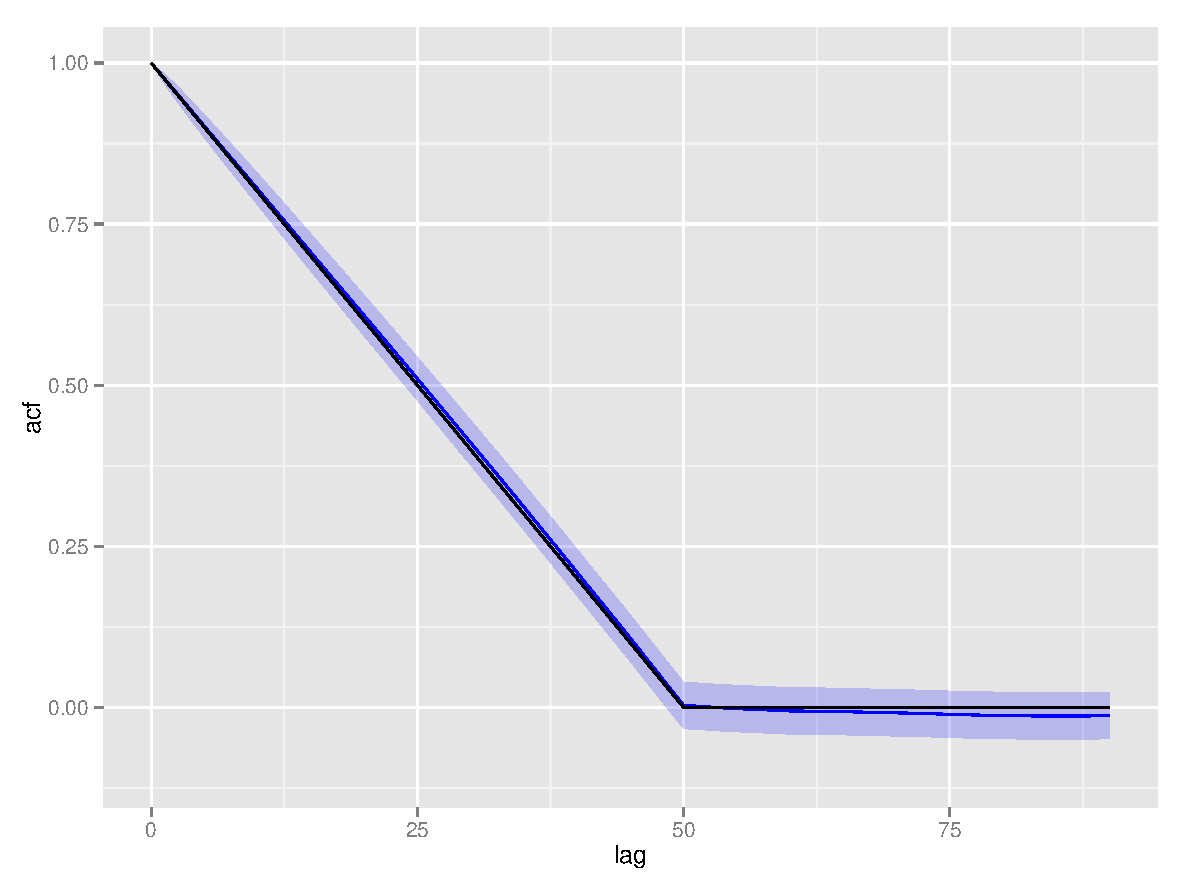
\includegraphics[width=\textwidth]{acfcth1}
   \caption{ACF of $Y_t(\theta =1, T_c=50)$ realization}
   \label{fig:acfcth1} 
\end{figure}
On Figure~\ref{fig:acfcth1} sample and theoretic ACFs of $Y_t$ realization with $T_c=50$ and $\theta=1$ are depicted (blue and black line respectively), as well as confidence intervals of sample ACF for any given lag (blue shade)\footnote{This legend applies to Figures \ref{fig:acfc}, \ref{fig:acfuth1}, and \ref{fig:acfu} as well.}. However, this realization of $Y_t$ is of little interest because it represents a market without any presence of traders who behave differently from LT. The next figure depicts a realization of $Y_t$ with $\theta=.7$.
\begin{figure}[h]
  \centering
    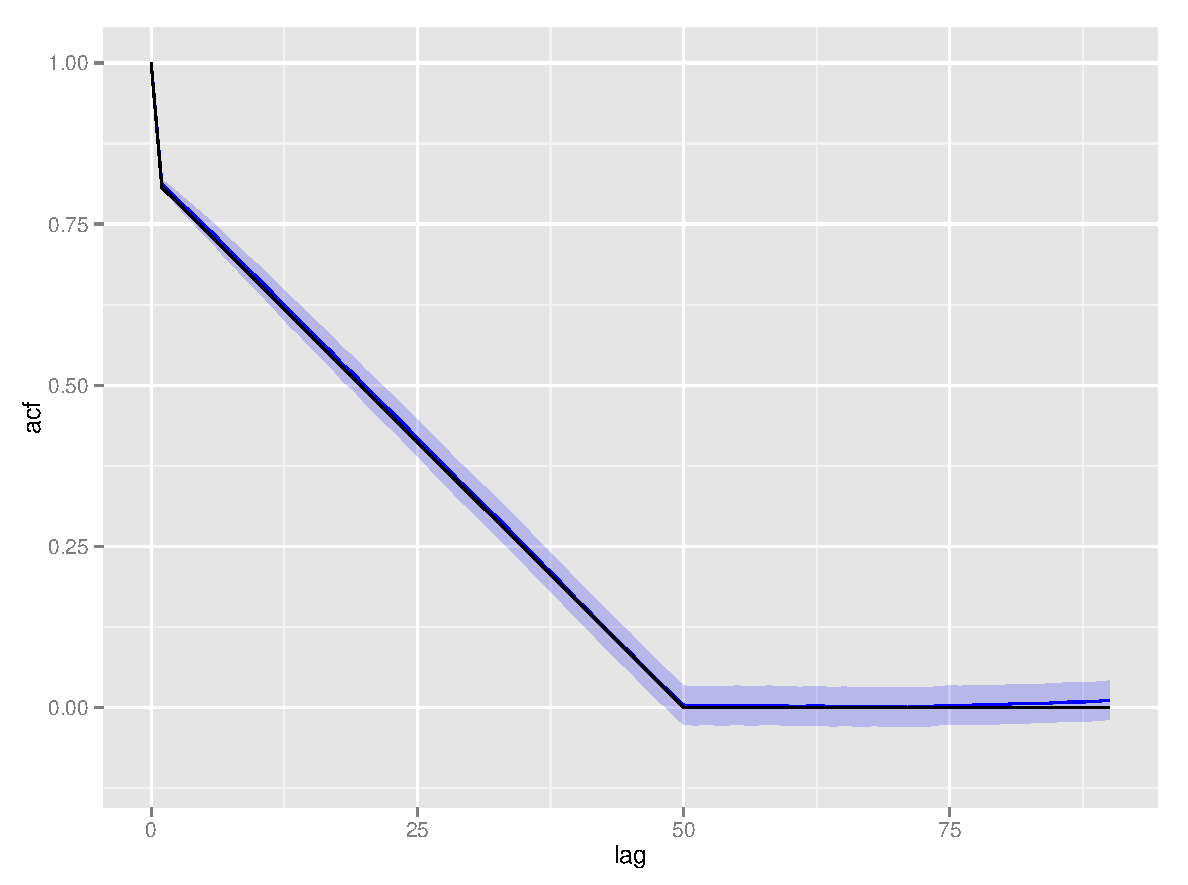
\includegraphics[width=\textwidth]{acfc}
   \caption{ACF of $Y_t(\theta =.7,\ T_c=50)$ realization}
   \label{fig:acfc} 
\end{figure}
Figure~\ref{fig:acfc} represents ACF of $Y_t$ realized with $\theta$ set to 0.7. As one can see, smaller $\theta$ "compresses" ACF along the y-axis by the rate $\frac{Var(Y_t|\theta=1)}{Var(Y_t|\theta=a)}$ for any $a \in (0,1]$. It is also important to note that this rate holds at any chosen lag $\Delta$ and any distribution of T.
\newpage
\subsection{Uniformly distributed T}
In this subsection it is assumed that $T_x$ is distributed uniformly on the interval $[\overline{T}-\delta,\overline{T}+\delta]$, where $\overline{T}>\delta$. It is more convenient to firstly consider how the expected value integrals from Formula \eqref{acorfinal} will change in this case. In order to do this, we must rewrite $E(\frac{\mathds{1}_{t+\Delta\leq T_x+x}}{T_x^2})$ for uniform distribution:
\begin{equation*}
\begin{gathered}
E\left(\frac{\mathds{1}_{t+\Delta\leq T_x+x}}{T_x^2}\right)=
\int_{\overline{T}-\delta}^{\overline{T}+\delta}\frac{\mathds{1}_{t+\Delta\leq T_x+x}}{2\delta T_x^2}dT_x
\end{gathered}
\end{equation*}
It is convenient to get rid of the indicator in the formula above. It can be done by explicitly stating possible relation between the limits of the $T_x$ domain and $t+\Delta-x$:
\begin{enumerate}
\item $t+\Delta-x<\overline{T}-\delta$\\
In this case we can replace the indicator with 1, because its argument holds within the whole domain of $T_x$. Thus, we get:
\begin{equation*}
\int_{\overline{T}-\delta}^{\overline{T}+\delta}\frac{1}{2\delta T_x^2}dT_x=\frac{1}{\overline{T}^2-\delta^2}
\end{equation*}
\item $\overline{T}-\delta\leq t+\Delta-x\leq\overline{T}+\delta$\\
Here we replace $\overline{T}-\delta$ with $t+\Delta-x$:
\begin{equation*}
\int_{t+\Delta-x}^{\overline{T}+\delta}\frac{1}{2\delta T_x^2}dT_x=\frac{\overline{T}+\delta-(t+\Delta-x)}{2\delta(\overline{T}+\delta)(t+\Delta-x)}
\end{equation*}
\item $\overline{T}+\delta<t+\Delta-x$, which yields 0.
\end{enumerate}
Transforming every condition above we split integrals from \eqref{acorfinal} into "subintegrals":
\begin{equation*}
\begin{gathered}
\int\limits^t_{t+\Delta-(\overline{T}-\delta)}\frac{1}{\overline{T}^2-\delta^2}dx+\int\limits^{t+\Delta-(\overline{T}-\delta)}_{t+\Delta-(\overline{T}+\delta)}\frac{\overline{T}+\delta-(t+\Delta-x)}{2\delta(\overline{T}+\delta)(t+\Delta-x)}dx,
\end{gathered}
\end{equation*}
for the numerator. In case of $\Delta>\overline{T}-\delta$ it becomes:
\begin{equation*}
\begin{gathered}
\int\limits^{t}_{t+\Delta-(\overline{T}+\delta)}\frac{\overline{T}+\delta-(t+\Delta-x)}{2\delta(\overline{T}+\delta)(t+\Delta-x)}dx
\end{gathered}
\end{equation*}
And, finally, for $\Delta>\overline{T}+\delta$ it becomes 0.

For the integral in the denominator of \eqref{acorfinal} this formula is slightly different:
\begin{equation*}
\begin{gathered}
\int\limits^t_{t-(\overline{T}-\delta)}\frac{1}{\overline{T}^2-\delta^2}dx+\int\limits^{t-(\overline{T}-\delta)}_{t-(\overline{T}+\delta)}\frac{\overline{T}+\delta-(t-x)}{2\delta(\overline{T}+\delta)(t-x)}dx
\end{gathered}
\end{equation*}
By calculating the integrals above we get:
\begin{equation}\label{acorunif}
\begin{cases}
\frac{ln\frac{\overline{T}+\delta}{\overline{T}-\delta}-\frac{2\delta}{\overline{T}^2-\delta^2}\Delta}{ln\frac{\overline{T}+\delta}{\overline{T}-\delta}+2\delta\frac{1-\theta}{\theta}\frac{\sigma^2_{NT}}{\sigma^2_{LT}}},\ \Delta<\overline{T}-\delta\\
\frac{\frac{\Delta}{\overline{T}+\delta}-(ln\frac{\Delta}{\overline{T}+\delta}+1)}{ln\frac{\overline{T}+\delta}{\overline{T}-\delta}+2\delta\frac{1-\theta}{\theta}\frac{\sigma^2_{NT}}{\sigma^2_{LT}}}, \Delta\in[\overline{T}-\delta;\overline{T}+\delta]\\
0, \Delta>\overline{T}+\delta
\end{cases}
\end{equation}
Figures \ref{fig:acfuth1} and \ref{fig:acfu} depict ACF of $Y_t$ given $T_x\sim U[30,70]$ and $\theta$ is equal to 1 and 0.7 respectively.

It is evident from the plots that our analytic result indeed lies within the confidence intervals and true ACF and its sampled counterpart diverge only when sufficiently high lags are considered, which is normal for this test.
\begin{figure}[H]
  \centering
    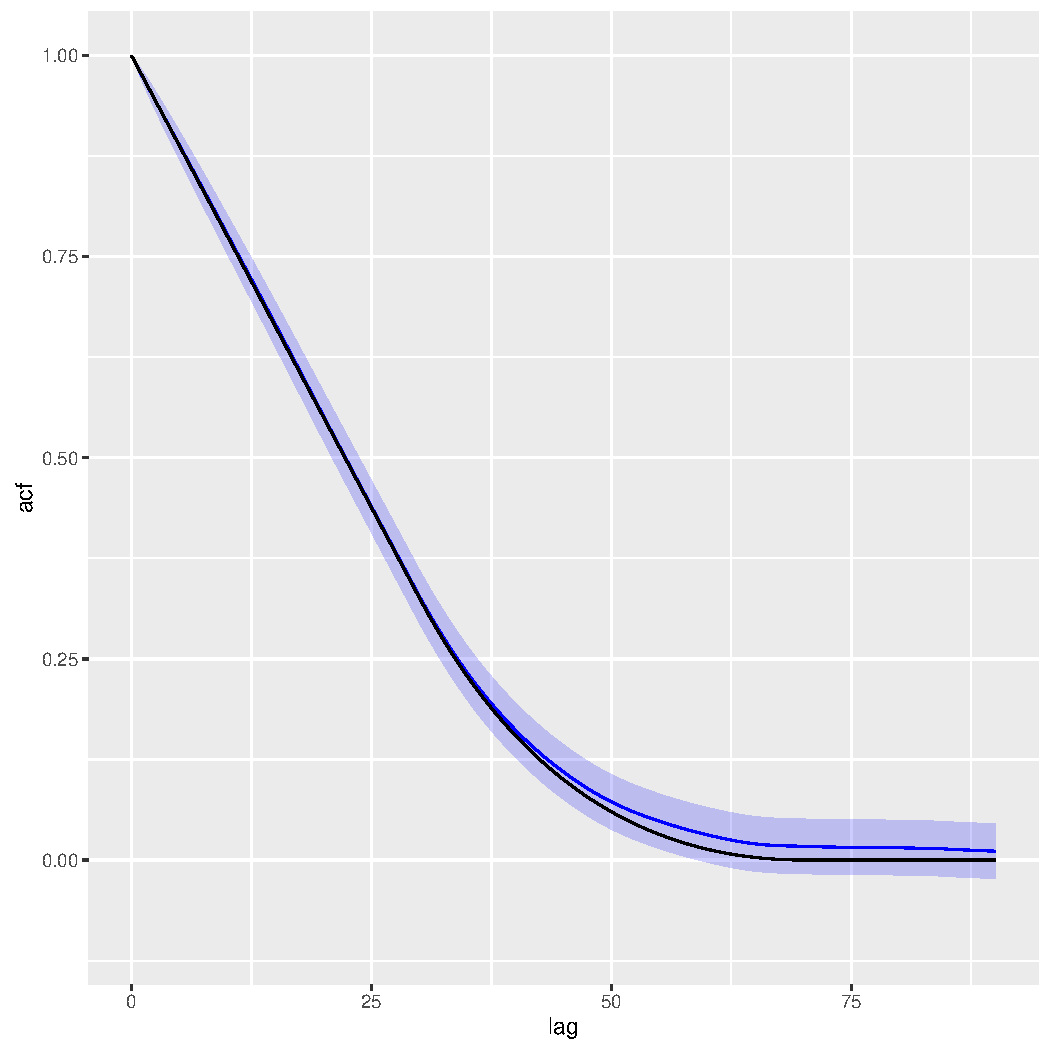
\includegraphics[width=\textwidth]{acfuth1}
   \caption{ACF of $Y_t(\theta =1, T_x\sim U[30,70])$ realization}\label{fig:acfuth1}  
\end{figure}
This method was tested for cherry-picked $T_x$ distributions that can be called the simplest relevant cases possible. Unfortunately, it becomes increasingly difficult to calculate the result for \eqref{acorfinal} for more complex distribution functions, so it stayed out of the scope of this work.
\begin{figure}[H]
  \centering
    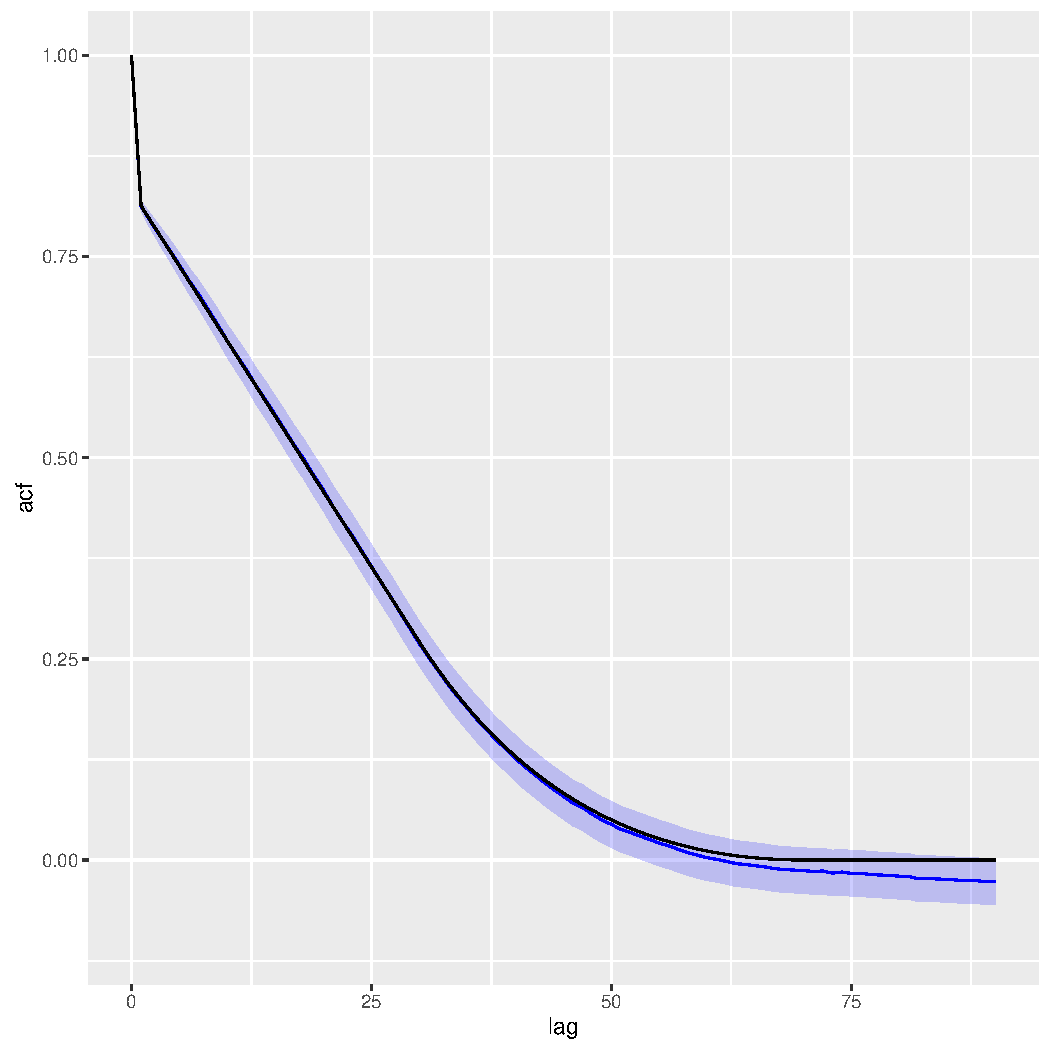
\includegraphics[width=\textwidth]{acfu}
   \caption{ACF of $Y_t(\theta =0.7, T=unif(30,70))$ realization}\label{fig:acfu}  
\end{figure}
However, the assumptions made are too strong for the real world. Certain caveats of this approach and ways to further improve the model are discussed in the next section.
\newpage

\section{Discussion}\label{sec:disc}
\subsection{Assumptions about RV distributions}
Some of the steps of this study required certain weak assumptions to make calculations easier. For example, Formula \eqref{acorfinal} was simplified as if $T_x$ had an upper limit well within $t$. It is not necessarily true, because institutional traders can stretch their execution time frame at least to a few days, which makes the approach discussed above unreliable. However, it can be mitigated using proper econometric techniques.

It is a lot more problematic to assume that the distributions (or, particularly, their moments) do not change within $t$. It is commonly known that the average number of transactions changes even throughout a day. Thus, it affects at least $\lambda$ and, likely, $\theta$, even considering the fact that the latter is supposed to capture changes \textit{in the breakdown of trade flows.} 

Despite the fact that it was stated when we were defining autocovariance of or process in \eqref{one}, it is still worth mentioning that distributions of traders' targets depend on trading signals. Signal $\xi_0$ implies that the expected value of an arbitrary transaction is 0. But any relevant announcement changes the initial signal and, therefore, the expected value of a transaction. An example of this is an increased demand for a stock when a positive news is comes out. 

While risks of strong assumptions about underlying random variables do not pose an obvious significant threat for the results, the conjecture about the linearity of trading strategies may prove far more detrimental to our methodology. The next subsection is devoted to this caveat.
\subsection{Choice of LT strategies}
The assumption about the "na\"iveness" of liquidity traders was made to show an illustrative example of results of our model. However, it is obvious that it is far from reality. One of the fundamental studies regarding how institutional traders choose their trading trajectory was conducted in Almgren/Chriss (2000). They use dynamic optimization procedure to minimize losses related to "reshuffling" one's portfolio (implementation shortfall). In spite of the fact that Almgren and Chriss considered only a single active trader, we deem this approach optimal for this work. 

Both in our study and in Almgren/Chriss (2000) trader's ability to estimate market variables (e.g., price impact and volatility) is "flawless". This can be overcome by assuming that trader's estimates are noisy, but the assumption of these estimates being unbiased is still vital.
\newpage

\section{Conclusions}\label{sec:concl}
In this study we proposed an approach to measure the intensity of liquidity trading using sampled ACF of trading volume under certain assumptions about the nature of interactions within a market. For the simplest cases this approach has proven to be useful, assuming that both researcher and trader gain same results from market variables estimation procedure.

However, this study has certain limitations. First of all, measuring errors in market variables estimates are not accounted for. Moreover, distributions of these variables do not change over time, which is too strong to be reliable. 

Secondly, the choice of the functional form of trading strategies was intentionally simplistic in order to illustrate the methodology. The best alternative is to use an approach analogous to Almgren/Chriss (2000). Solving the problem stated in their work with setting adjustments from our paper deserves a separate study and therefore remains out of the scope.

Finally, even knowing outcomes of optimization, one must correctly trace trading trajectories of market participants from real data. An example of this necessity is estimation of execution time distribution. 
\newpage
%change eqrefs to Eq. instead of Formula
\section{References}\label{sec:ref}
\printbibliography
\newpage

\appendix
\end{document}
